\documentclass{article}

\usepackage{tikz}
\usepackage{tikz}
\usepackage{pgfplots}
\usetikzlibrary{backgrounds, positioning, fit}
\usetikzlibrary{shapes.geometric}
\usetikzlibrary{patterns}

%% put tikzlibrary below if necessary

% set up externalization
\usetikzlibrary{external}
\tikzset{external/system call={latex \tikzexternalcheckshellescape -halt-on-error
-interaction=batchmode -jobname "\image" "\texsource";
dvips -o "\image".ps "\image".dvi;
ps2eps "\image.ps"}}
\tikzexternalize



\begin{document}

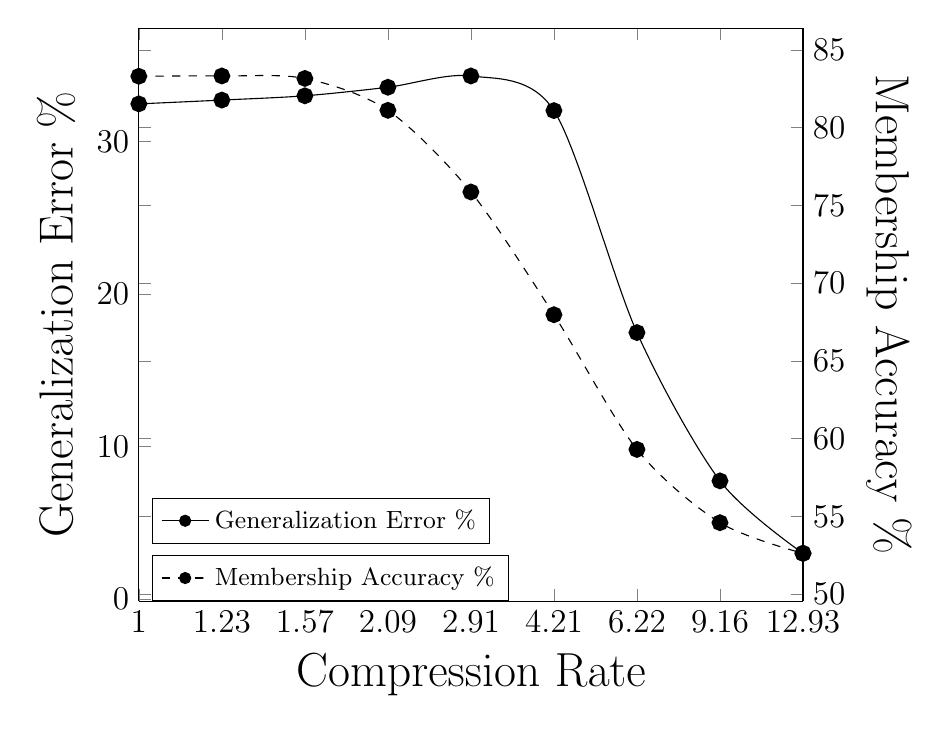
\begin{tikzpicture}
% let both axes use the same layers
\pgfplotsset{set layers}
%
\begin{axis}[
%title={(c) Location},
%title style={at={(0.5,0)},anchor=north,yshift=-40, font=\huge},
scale only axis,
line width=2.0pt,
mark size=2.0pt,
xmin=0,xmax=8,
ylabel={Generalization Error \%},
axis y line*=left,
xlabel={Compression Rate},
xlabel style={font=\LARGE},
ylabel style = {font=\LARGE},
xticklabel style = {font=\large},
yticklabel style = {font=\large},
xtick={0,1,2,3,4,5,6,7,8},
xticklabels={1, 1.23, 1.57, 2.09, 2.91, 4.21, 6.22, 9.16, 12.93},
legend style={at={(0.02,0.1)},anchor=south west, font=\small}
]
\addplot[
    color=black,
    solid,
    mark=*,
    mark options={solid},
    smooth
    ]
    coordinates {
    (0,32.47)(1,32.72)(2,33)(3,33.56)(4,34.3)(5,32.03)(6,17.48)(7,7.76)(8,3.01)
      };
\addlegendimage{color=black,solid,mark=*, mark options={solid}}
\addlegendentry{Generalization Error \%}
\end{axis}

\begin{axis}[
scale only axis,
line width=2.0pt,
mark size=2.0pt,
xmin=0,xmax=8,
ylabel near ticks, yticklabel pos=right,
ylabel={Membership Accuracy \%},
ylabel style = {rotate=180,font=\LARGE},
yticklabel style = {font=\large},
axis x line=none,
legend style={at={(0.02,0)},anchor=south west, font=\small}
]
\addplot[
    color=black,
    dashed,
    mark=*,
    mark options={solid},
    smooth
    ]
    coordinates {
    (0,83.30)(1,83.32)(2,83.16)(3,81.11)(4,75.86)(5,67.97)(6,59.31)(7,54.60)(8,52.63)
        };
\addlegendimage{color=black,dashed,mark=*,mark options={solid}}
\addlegendentry{Membership Accuracy \%}
\end{axis}
\end{tikzpicture}



\end{document}
